%%
%% This is file `sample-sigconf.tex',
%% generated with the docstrip utility.
%%
%% The original source files were:
%%
%% samples.dtx  (with options: `sigconf')
%% 
%% IMPORTANT NOTICE:
%% 
%% For the copyright see the source file.
%% 
%% Any modified versions of this file must be renamed
%% with new filenames distinct from sample-sigconf.tex.
%% 
%% For distribution of the original source see the terms
%% for copying and modification in the file samples.dtx.
%% 
%% This generated file may be distributed as long as the
%% original source files, as listed above, are part of the
%% same distribution. (The sources need not necessarily be
%% in the same archive or directory.)
%%
%% The first command in your LaTeX source must be the \documentclass command.
\documentclass[sigconf]{acmart}

%%
%% \BibTeX command to typeset BibTeX logo in the docs
\AtBeginDocument{%
  \providecommand\BibTeX{{%
    \normalfont B\kern-0.5em{\scshape i\kern-0.25em b}\kern-0.8em\TeX}}}

%% Rights management information.  This information is sent to you
%% when you complete the rights form.  These commands have SAMPLE
%% values in them; it is your responsibility as an author to replace
%% the commands and values with those provided to you when you
%% complete the rights form.
\setcopyright{acmcopyright}
\copyrightyear{2018}
\acmYear{2018}
\acmDOI{10.1145/1122445.1122456}

%% These commands are for a PROCEEDINGS abstract or paper.
\acmConference[WebSci '21]{WebScie '21: ACM Web Science Conference}{June 21--25, 2021}{University of Southampton, UK}
\acmBooktitle{WebSci '21: ACM Web Science Conference,
  June 21--25, 2021, University of Southampton, UK}
%%\acmPrice{15.00}
%%\acmISBN{978-1-4503-XXXX-X/18/06}


%%
%% Submission ID.
%% Use this when submitting an article to a sponsored event. You'll
%% receive a unique submission ID from the organizers
%% of the event, and this ID should be used as the parameter to this command.
%%\acmSubmissionID{123-A56-BU3}

%%
%% The majority of ACM publications use numbered citations and
%% references.  The command \citestyle{authoryear} switches to the
%% "author year" style.
%%
%% If you are preparing content for an event
%% sponsored by ACM SIGGRAPH, you must use the "author year" style of
%% citations and references.
%% Uncommenting
%% the next command will enable that style.
%%\citestyle{acmauthoryear}

%%
%% end of the preamble, start of the body of the document source.
\begin{document}

%%
%% The "title" command has an optional parameter,
%% allowing the author to define a "short title" to be used in page headers.
\title{Material and immaterial regional interdependencies: using the web to predict regional trade flows}

%%
%% The "author" command and its associated commands are used to define
%% the authors and their affiliations.
%% Of note is the shared affiliation of the first two authors, and the
%% "authornote" and "authornotemark" commands
%% used to denote shared contribution to the research.
\author{Emmanouil Tranos}
%%\authornote{Both authors contributed equally to this research.}
\email{e.tranos@bristol.ac.uk}
\orcid{0000-0002-9620-6542}
\affiliation{%
  \institution{University of Bristol and The Alan Turing Institute}
  %%\streetaddress{P.O. Box 1212}
  %%\city{Dublin}
  %%\state{Ohio}
  \country{UK}
  %%\postcode{43017-6221}
}

\author{Andre Carrascal Incera}
\email{carrascalandre@uniovi.es}
\affiliation{%
  \institution{University of Oviedo}
  %%\streetaddress{1 Th{\o}rv{\"a}ld Circle}
  %%\city{Hekla}
  \country{Spain}}


\author{George Willis}
\email{GCW519@student.bham.ac.uk}
\affiliation{%
  \institution{University of Birmingham}
  %%\city{Rocquencourt}
  \country{UK}
}


%%
%% By default, the full list of authors will be used in the page
%% headers. Often, this list is too long, and will overlap
%% other information printed in the page headers. This command allows
%% the author to define a more concise list
%% of authors' names for this purpose.
\renewcommand{\shortauthors}{Tranos, et al.}

%%
%% The abstract is a short summary of the work to be presented in the
%% article.
\begin{abstract}
  This paper brings new web data and machine learning methods in order to expose the structure and the evolution of regional trade interdependencies. Although our focus is on the UK regions, the proposed research framework lends itself to applications to other countries. Interregional trade relationships have traditionally been very difficult to capture, as national statistics do not monitor intra-country trade links at the firm level. Recently, the EUREGIO project (Thissen et al., 2018) has published spatially disaggregated Input-Output (I-O) information for 37 NUTS2 UK regions for 14 industries, which includes imports and exports by region of origin and destination. This database was developed using the interregional trade data from the PBL Netherlands Environmental Assessment Agency, freight transport data from Eurostat (for goods), and business flight ticket information (for services). Nevertheless, building such an interregional trade dataset has been a costly and non-trivial process. In this paper, we are proposing a new research framework to predict such flows by utilising freely available web data. Specifically, we are employing the JISC UK Web Domain Dataset in order to extract hyperlinks between geolocated commercial websites in the UK. This dataset is a subset of the Internet Archive, which includes all the archived webpages under the .uk country code Top Level Domain (ccTLD). We are able to geolocate these webpages by searching the archived web text for the inclusion of a UK postcode. In addition, this dataset also contains the hyperlinks included in the archived webpages and we are able to aggregate these data and create an interregional network based on the hyperlinks between geolocated commercial webpages. Formally, we approach the prediction of the trade flows as a regression problem. Hence, we employ some well-established machine learning models, such as Random Forests, to predict interregional trade flows using, among other features, the network of digital interdependencies between the UK regions. Our results indicate a very high capacity of the interregional hyperlinks feature to predict interregional trade indicating that trade leaves behind significant digital breadcrumbs.
\end{abstract}

%%
%% The code below is generated by the tool at http://dl.acm.org/ccs.cfm.
%% Please copy and paste the code instead of the example below.
%%
\begin{CCSXML}
	<ccs2012>
	<concept>
	<concept_id>10002951.10003260.10003277</concept_id>
	<concept_desc>Information systems~Web mining</concept_desc>
	<concept_significance>500</concept_significance>
	</concept>
	<concept>
	<concept_id>10010405.10010476.10003392</concept_id>
	<concept_desc>Applied computing~Digital libraries and archives</concept_desc>
	<concept_significance>500</concept_significance>
	</concept>
	</ccs2012>
\end{CCSXML}

\ccsdesc[500]{Information systems~Web mining}
\ccsdesc[500]{Applied computing~Digital libraries and archives}

%%
%% Keywords. The author(s) should pick words that accurately describe
%% the work being presented. Separate the keywords with commas.
\keywords{interregional trade, web archives, web data, machine learning, prediction, random
	forests}

%% A "teaser" image appears between the author and affiliation
%% information and the body of the document, and typically spans the
%% page.
%%\begin{teaserfigure}
%%  
\includegraphics[width=\textwidth]{sampleteaser}
%%  \caption{Seattle Mariners at Spring Training, 2010.}
%%  \Description{Enjoying the baseball game from the third-base
%%  seats. Ichiro Suzuki preparing to bat.}
%%  \label{fig:teaser}
%% \end{teaserfigure}

%%
%% This command processes the author and affiliation and title
%% information and builds the first part of the formatted document.
\maketitle

\hypertarget{sec:1}{%
	\section{Introduction}\label{sec:1}}

Bilateral trade is a complex phenomenon per se \citep{topology_trade},
but its complexity increases when it is approached from a spatially
disaggregated perspective. Regions\footnote{In the paper we shall use
	the terms `regional' and `subnational' interchangeably.} behave
different from countries from an economic perspective as they are more
specialised in specific sectors and more open to trade with other
regions in comparison to national economies. This
makes them face very important external dependencies. Also, regions vary
greatly in terms of their specialisation patterns, and therefore, there
is great variation in terms of trade relationships and openness within
regions. Furthermore, because of globalisation patterns and the spatial
fragmentation of production, regional trade of intermediate and final
products is no longer constrained to interregional transactions within
countries. So, by lowering trade barriers in the past decades,
restrictions to international trade declined and the external dependence
of regions became global. Events happening in regions of countries from
the other side of the globe can affect closer regions through
disruptions in Global Supply Chains, as the Covid-19 crisis is showing
us. A region would be affected by an economic downturn in a second
region if it sells much of its production to that region (directly), or
if it sells its production to regions that sell their production to that
region (indirectly), while regions less dependent on that second region
might be hurt to a much lesser extent when in crisis
\citep{thissen2016competitive}. This is why, among other factors,
regions had significantly divergent experiences in avoiding or
overcoming economic shocks \citep{kitsos2019role}.

Consequently, understanding and, if possible, predicting regional trade
is key to comprehend regional economic performance and the exposure to
internal and external shocks, but also to articulate proper place-based
development policies \citep{barca2009agenda}. Interregional relations
and modern supply chains are central in a systemic way of thinking about
regional innovation and growth strategies \citep{thissen2013integrated}
such as the smart specialisation policy initiatives
\citep{mccann2015smart}.

The big caveat is the lack of sectoral, interregional trade data, which
are absent from key cross-country data providers such as the Eurostat
and OECD. One exception is the work of \citet{thissen2013integrated},
who followed the parameter-free \citet{simini2012universal} approach and
estimated interregional trade flows between 256 European NUTS2 regions
at a sector level by disaggregating national input-output tables. These
data have been utilised in regional economics research -- see discussion
and references in Section \protect\hyperlink{sec:4}{4} -- and are
nowadays the go-to interregional trade data set. Nevertheless,
production of such data are neither simple nor easily reproduced.

Our paper contributes to this line of inquiry by utilising
state-of-the-art machine learning algorithms and novel web data to make
out-of-sample predictions for the UK NUTS2 regions during the period
\(2000\)-\(2010\). Specifically, we use open and archived web data to
create counts of hyperlinks between websites that we are able to
geolocate. We feed such variables to a Random Forest (RF) model,
alongside a limited number of other predictors, and we are able to
achieve accuracy scores above 90\% in predicting \emph{unseen}
interregional trade flows. Our underpinning hypothesis is that trade
leaves behind digital breadcrumbs (\citet{rabari_storper2014}), which
can be effectively utilised to predict interregional trade flows, which
are both important for regional policies and also very difficult to
observe.

Modelling interregional trade flows has traditionally been within the
core of geographical research as it well embedded within the
discipline's effort to explain the determinants of aggregated
interactions across space \citep[for a recent review
see][]{oshan2020spatial}. Methodological and conceptual developments on
\emph{spatial interaction models} have been extensively employed in
order to model flows of trade between regions
\citep[\citet{paul2008incorporating}]{chun2012modeling} and countries
\citep{de2017testing, de2017competing}. Following current debates within
the quantitative geographical thinking \citep{singleton2021geographic}
and, more broadly, computational social sciences
\citep{lazer2009social}, geographical research has been focusing more on
explaining the determinants of interregional trade flows than predicting
such flows.

This paper is aligned with the state-of-art within the Data Science
research domain and its subsequent epistimological effects in geography
\citep{singleton2021geographic, creditspatial} and economics
\citep{kleinberg2015prediction} regarding the role of machine learning
algorithms in making out-of-sample predictions of data instead of
focusing on explanatory research frameworks. Simply put, the above
advocate towards the use of ML algorithms, such as RF, as they
outperform ordinary least squares -- still one of the widely used
estimators to model interregional trade flows -- in out-of-sample
predictions even when using moderate size training datasets and limited
number of predictors \citep{mullainathan2017machine, athey2019machine}.
Such an approach can be particularly useful for predicting interregional
trade flow given the scarcity and cost to produce such data.

RF have been extensively utilised in answering regression type of
problems. \citet{pourebrahim2019trip} coupled a traditional
methodological framework -- gravity and spatial interaction modelling --
with ML techniques including RF as well as data from online social media
to predict commuting flows in New York City. \citet{lima2020predicting}
used ML and RF to predict and explain corruption across countries.
\citet{sinha2019assessing} open a dialogue on the need for spatial
ensemble learning approaches, such as RF, aimed to be used with spatial
data with high autocorrelation and heterogeneity. \citet{creditspatial}
introduced spatially explicit RF to predict employment density in Los
Angeles. \citet{guns2014recommending} use RF to predict and recommend
high-potential research collaborations, which have not yet been
materialised.\\
\citet{ren2019predicting} train RF as well as other classifiers to
predict socio-economic status or cities using a variety of online and
mobility predictors. \citet{wang2017structure} train RF and other
machine learning algorithms to predict urban socio-economic
characteristic based on 311 service requests\footnote{these are
	non-emergency urban requests or complaints reported to the 311 phone
	number}. RF tend to perform better than other algorithms in
predicting, for example, real estate prices, income per capita,
percentage of residents with a graduate degree, percentage of unemployed
residents, percentage of residents living below the poverty level, as
well as demographic characteristics for 30 US cities.

The structure of the paper goes as following. The next section reviews
the literature which either highlighted the lack of interregional trade
data or employed innovative and often data-intensive approaches to
capture such flows. Then, we describe the methods and the data we use
and present the results of the analysis. The paper ends with a
conclusions section.

\hypertarget{sec:2}{%
	\section{From the lack of regional trade data to webdata}\label{sec:2}}

The lack of bilateral trade data resulted in a very prolific branch of
the literature attempting to estimate trade flows at country and
regional level. Without a doubt, the most important step in this regard
was the introduction of gravity equations in the early works of
\citet{tinbergen1962shaping}, \citet{linnemann1966econometric} and
\citet{leamer1r}. In summary, a gravity equation is based on the idea
that bilateral trade between two territories depends on their sizes
(expressed normally as GDP or GDP per capita) in relation to the
distance between them or transport costs (as an impediment factor), and
some preference factors (common border, common language, etc.)
\citep{egger2002econometric, anderson2003gravity}. In the last years,
the emphasis has been placed on discussing the proper estimation methods
to accurately predict trade flows (OLS, Tobit, panel fixed effects,
Heckman two-step, etc.). A review of the alternative methods applied in
gravity models can be seen in \citet{gomez2013comparing}.

A different strand of the literature comes from the multisectoral trade
analysis of Input-Output flows. While the theoretical framework of
multiregional Input-Output databases was developed in the 1950s
\citep{isard1956location}, the biggest empirical take-off did not come
until the release of the World Trade Organisation databases such as the
WIOD (World Input-Output Database)
\citep{dietzenbacher2013construction}. The availability of a series of
homogeneous tables describing sectoral trade flows within and between
countries was a significant factor behind the revitalisation of the
global value chains and defragmentation studies
\citep{timmer2015illustrated, los2015global, los2016tracing, antras2018measurement},
as well as for the analysis of the global environmental footprints
\citep{arto2014comparing, owen2016explaining}.

Still, those global databases based on official national accounting data
(survey) are only available at the country level, and researchers and
statistical offices that want to use a multi-regional Input-Output model
at a subnational level need to estimate such interregional flows between
sectors and regions within a country. Several non-survey methods were
developed with that aim, among them the ones based on location
quotients, the cross-hauling adjusted regionalisaation method (CHARM),
and entropy methods. They all rely on structural macroeconomics
identities in order to be consistent with the total volumes coming from
the known regional figures and with the sector-by-sector framework.
Examples of this are the works by \citet{sargento2012inter},
\citet{tobben2015construction} or \citet{boero2018regional}, among many
others.

More related to the focus of this paper, \citet{hellmanzik2016gravity}
and \citet{hellmanzik2017taking} explored the role of `virtual'
proximity in explaining the trade in services between countries and
their international financial integration. Both papers used data from
\citet{chung2011geography}, who utilised the universe of the Yahoo
indexed websites from 2003 and 2009: 33.8 billion websites from 273
different country top-level domains (ccTLD). They mined these data and
identified 9.3 billion hyperlinks between these websites. The
aggregation of these bilateral hyperlinks at country level was termed as
virtual proximity. Following \citet{kimura2006gravity},
\citet{hellmanzik2016gravity} and \citet{hellmanzik2017taking} estimated
gravity models to test whether international trade is associated with
the volume of hyperlinks between countries. Their results indicated that
indeed, the aggregated volume of hyperlinks between countries is\\
a significant determinant of services trade and its effect is
particularly large for finance services, but also for communications,
insurance, IT and audio-visual services. Government and construction
trade services, on the other hand, appear to be less associated with
virtual proximity. In any case, their findings illustrate how virtual
proximity may reduce the negative effects of distance, providing a
possible explanation for the decline in the distance effect on
international services trade found by \citet{head2009remote}.

Web data have been utilised before in order to study spatial
relationships. Recently, \citet{meijers2019using} proposed the `toponym
co-occurrence approach' to study intercity relationships. Their study is
based on retrieving relevant information from text corpora by
considering when places (i.e.~toponyms) are mentioned together in the
same website. Then, they employ machine learning techniques to
understand the context within which these place toponyms co-occurred and
cluster these relationships. Their results reflect the spatial
interdependencies within the Dutch settlement system and illustrate the
utility of web data to capture such spatial relationships and complement
existing relational data sources or substitute the lack of such data. In
a similar manner, \citet{devriendt2008cyberplace} and
\citet{janc2015visibility} had employed the Google search engine to
create counts of webpages which mentioned pairs of cities in order to
build urban connectivity measures.

Other researchers focused on more handpicked subsets of the web.
\citet{kessler2017extracting} and \citet{salvini2016spatialization}
employed the Wikipedia as their means to study spatial relationships.
While the former used the hyperlinks between German Wikipedia webpages
to represent the hierarchy of urban centres in Germany, the latter
utilised the English Wikipedia to build a graph of world cities.
\citet{lin2007blog} used hyperlinks from US-based webblogs to analyse
the spatial reflections of the blogsphere. In the same vein,
\citet{jones2010blog} used hyperlinks between webblogs focused on the
New York City theater scene to investigate the existence and role of a
`virtual buzz'. A number of studies utilised hyperlinks between and to
administrative websites to study spatial relationships and structure
\citep{holmberg2009local, holmberg2010co, janc2015geography}.

Studying university websites and their hyperlinks is a popular
application of \emph{webometrics}, or, in other words, ``the
quantitative study of {[}w{]}eb-related phenomena''
\citet{thelwall_webometrics}. Early work from Thelwall
\citep{thelwall2002top, thelwall2002evidence} analysed the distribution
of hyperlinks between university websites and the role geography plays
in how universities establish hyperlinks. Ortega and Aguillo
\citetext{\citeyear{ortega2008linking}; \citeyear{ortega2008visualization}; \citeyear{ortega2009mapping}}
broaden the scale of analysis focusing on universities from Europe and
around the world. More recently, \citet{hale2014mapping} using the same
data employed for this paper analysed the graph of hyperlinks between UK
university websites. Reflecting earlier results, their analysis
highlighted the role of distance in establishing hyperlinks contrary to
league table rankings, which do not seem to drive such linkages.

The association of physical distance with the distribution of hyperlinks
was the focus of the earliest, to our knowledge, application of
webometrics on studying spatial relationships. Using a limited sample of
websites, \citet{halavais2000national} indicated that hyperlinks tend to
follow national borders and gravitate towards the US.

The use of web data has also been employed to answer business related
research questions. \citet{vaughan2006hyperlinks} studied hyperlinks to
business websites and found that most such links reflect business
motivations and contain useful business information. Nevertheless, they
observed scarcity of links to competitors. Other studies found
significant correlations between the number of incoming links and
business performance \citep{vaughan2004exploring, vaughan2004links}.
More recently, \citet{kruger2020digital} used hyperlinks between
business websites in Germany to test the role of different proximity
frameworks, which were operationalised using hyperlinks data, on the
innovative behaviour of these firms. Their results indicated that
innovative businesses share more hyperlinks with other business, which
also tend to be innovative. Moreover, innovative businesses are being
located in dense urban areas and share hyperlinks with websites from
remote businesses.

In summary, the scarce of bilateral regional trade data is a
well-established problem in the relevant literature. Research has done
some first steps towards employing the wealth of web data in order to
capture country-to-country trade relationships. Such approaches
capitalised the tradition of webometrics research, which has also been
focusing on illustrating spatial relationships. Building upon such
studies, this paper aims to address the lack of regional trade data
problem by employing open and underutilised data from web archives.
Importantly, we do this within a modern ML framework, which is described
in the next section.

\hypertarget{sec:3}{%
	\section{Methodological framework}\label{sec:3}}

The main method employed here to predict inter-regional trade flows is
Random Forests (RF). This is a widely used ML technique both for
regression and classification problems \citep{biau2012analysis}. It was
firstly introduced by \citet{breiman2001random} and since then its
popularity increases making it a standard tool for data science
problems. The benefits of RF include its capacity to handle skewed
distributions and outliers and to effectively model non-linear
relationships between the dependent and independent variables, the small
number of hyperparameters that need to be tuned, the low sensitivity
towards the values of these parameters as well as the relatively short
training time \citep{Caruana2008, liaw2002classification, yan2020using}.
Moreover, predictions based on RF are more accurate than those based on
single regression trees, can illustrate the predictor importance, are
fast and easy to implement
\citep{breiman2001random, sulaiman2011intelligent, pourebrahim2019trip, biau2012analysis}.
Current economic thinking advocates towards the use of RF as they tend
to outperform ordinary least squares in out-of-sample predictions even
when using moderate size training datasets and limited number of
predictors \citep{mullainathan2017machine, athey2019machine}.

RF is a tree-based ensemble learning method \citep{breiman2001random}.
It starts by creating random samples of the training data, which are
then used to grow an equivalent number of regression trees to predict
the dependent variable. This variable can be either a continuous one for
regression problems or a categorical one for classification problems.
Both observations and predictors are randomly sampled for the individual
trees. Importantly, no pruning is applied for the trees to fully grow.
Instead, these decision trees are trained in parallel on their own
sample of the training data created with bootstrapping. An essential
attribute of RF is their potential \emph{not} to overfit. The latter
refers to the capacity of a model to explain very well a specific
dataset, but not being able to generalise the learned patterns to an
unseen test dataset. Even though each tree on its own can overfit, the
forest -- i.e.~the ensemble of trees -- does not suffer from overfitting
because the individual tree errors are averaged to produce the error of
the overall forest leading also to decreased variance between trees
\citep{last2002improving}. To make a prediction for regression problems,
RF average the predictions of all decision trees. So, the trade flows
\(IO\) between regions \(i\) and \(j\) can be represented as:

\begin{align}
	f(X_{i}, X_{j}, Z_{ij}|\hat{\theta}|) = \frac{1}{B} \sum_{b = 1}^{B} \hat{T_{b}} \label{eq:trees}
\end{align}

where, \(X_{i}\), \(X_{j}\), and \(Z_{ij}\) are the origin \(i\),
destination \(j\) and origin-destination pair \(ij\) predictors of
regional trade respectively, \(\hat{\theta}\) is a vector of the
estimated hyperparameters, \(B\) is the total number of trees the RF
grew, which is also one of the estimated hyperparameters and
\(\hat{T_{b}}\) represents the prediction of each independent tree
\citep{yan2020using}.

To estimate RF models we employ the widely used \texttt{caret} package
for \texttt{R} \citep{kuhn2008building} and we build the following
\emph{rolling forecasting} workflow: \emph{(1)} train RF models on data
from years \(t\) and \(t + 1\) from the study period 2000-2010 to
increase the size of the training dataset; \emph{(2)} evaluate their
predictive capability using cross validation (CV); \emph{(3)} apply the
estimated RF models from step \emph{(1)} on unseen data from the
following years \((t + 2)\) to predict trade flows for that year and
evaluate their predictive capability of such unseen data.

We opted against pooling the data to maintain their temporal structure
both for methodological and conceptual reasons. Random sampling and
pooling may lead to utilise future values of hyperlink flows to predict
past regional trade flows, which might be counterintuitive.Instead, we
opted towards building biyearly RF modesl with 10-fold CV to assess
their predictive capability. To do so, we split the biyearly subsets of
the data in 10 random samples, trained a RF on the nine and tested its
predictive capacity on the holdout one.This process is repeated ten
times in order for all 10 samples to act as holdout ones. Then, the
predictive performance of the RF is equal to the mean performance of the
10 models. This workflow enables us to make out-of-sample predictions
and test our models and research framework in previously unseen data.
Successful predictions within this framework will illustrate the digital
traces that regional trade leaves behind and how useful such web data
are in predicting trade flow that we have little information about.

To assess the predictive capability of the models, we utilise three
broadly used metrics: mean absolute error (MAE), root mean square error
(RMSE) and the coefficient of determination (R squared):

\begin{align}
	R^2 = 1 - \frac{\sum_{k} (y_{k} - \hat{y_{k}})^2} {\sum_{k} (y_{k} - \overline{y_{k}})^2} \label{eq:rsquared}
\end{align}

\begin{align}
	MAE = \frac{1}{N} \sum_{k = 1}^{N} |\hat{y_{k}} - y_{k}| \label{eq:mae}
\end{align}

\begin{align}
	RMSE =  \sqrt{\frac{\sum_{k = 1}^{N} (\hat{y_{k}} - y_{k})^2} {N}} \label{eq:rmse}
\end{align} \(y_{k}\) is the \(k^{th}\) observation of the dataset,
which consists of \(N\) observation in total. \(\hat{y_{k}}\) is the
\(k_{th}\) predicted value for the dependent variable and
\(\overline{y_{k}}\) is the average value of \(y\). The last two metrics
are expressed in the same units as the dependent variable --
\(\pounds 100,000s\) -- while the first one is the coefficient of
determination between the observed and the predicted values of regional
trade flows. Regarding \(MAE\), it is the absolute difference between
the observed and the predicted trade flows. While \(MAE\) does not
penalise for large errors, \(RSME\) does so as it is proportional to the
squared difference between the observed and the predicted trade flows.
This means that larger errors carry more weight for \(RMSE\)
\citep{pontius2008components}.

RF allow to estimate the predictor importance. Using the built-in
bootstrapping procedure, MSE is recorded for each tree when including
all the predictors and then again by excluding one by one all the
predictors. The derived decrease in the MSE created by removing each
predictor signifies its importance in the model
\citep{breiman2001random}\footnote{see also the \texttt{randomForest}
	\texttt{R} package, which is based on Breiman's
	\citeyearpar{breiman2001random} original implementation}.

We then move to test the predictive capacity of RF trained on year \(t\)
and \(t + 1\) on unseen data from year \(t + 2\). This yearly data split
equites to a \emph{firewall principle} \citep{mullainathan2017machine},
which prevent data leakage between the training and the test dataset.
Being able to accurately predict unseen regional trade flows provides
further statistical evidence for the validity of for our proposed
research strategy. Moreover, it advocates towards the utility of our
research strategy and its applicability in predicting regional trade
flows.

Our research framework enables us to disaggregate the models based on
economic sectors and, therefore, we are able to further assess their
sensitivity. In addition, we utilise different subsets of the web data
as another robustness checks. The details of these data are exaplined in
the next section.

\hypertarget{sec:4}{%
	\section{Data}\label{sec:4}}

The hyperlinks data have been derived from the JISC UK Web Domain
Dataset\^{},
{[}\url{https://data.webarchive.org.uk/opendata/ukwa.ds.2/}{]}
\citep{ukwebarchive}, which contains all the archived .uk webpages
contained in the Internet Archive. These data have been utilised in
other studies which explored the role of online content of local
interest in attracting individuals online \citep{tranos2020individual}
and on the long term regional productivity effects of the early adoption
of web technologies \citep{tranos2020digital}.

In the case of the information on interregional trade, we obtain the
flows of imports and exports between the UK NUTS2 regions from the
EUREGIO database (\citet{thissen2018euregio}), which are the most
detailed data currently available about the economic and trade structure
of the UK and EU regions. The EUREGIO uses the World Input-Output
Database (WIOD) (\citet{timmer2015illustrated}) as a starting point and
adds regional detail for EU Member States as of 2010. The EUREGIO is
available for the years 2000 to 2010, and it contains information for
256 European NUTS2 regions and 14 sectors in each region
(\citet{ijtsma2020uk}).

Regional trade in the EUREGIO database is taken from the PBL Netherlands
Environmental Assessment Agency regional trade data for the year 2000 as
a prior to the estimations for the whole series 2000-2010
(\citet{thissen2013integrated} and \citet{thissen2013european}). The
PBL/RT dataset was constructed by merging data from several sources:
national accounts of the selected countries; international trade data on
goods from \citet{feenstra2005world} and on services from Eurostat;
macroeconomic regional data from Cambridge Econometrics and Eurostat's
regional accounts; information on freight transport among European
regions for approximating the network of trade in goods; and first and
business class airline tickets information for approximating the network
of trade in services. Therefore, in the EUREGIO database no spatial
structure has been imposed on the data, which means that no specific
model was used to estimate trade flows and patterns. The procedure used
allocates the trade over the regions depending on the amounts produced
and consumed in every region. The estimation approach ensures the final
consistency of the regional tables with the national tables
(\citet{thissen2018euregio}; \citet{ivanova2019regional}).

This database has been used recently in studies estimating the impacts
of different economic shocks. \citet{los2017mismatch}, paradoxically
found that those regions that voted in favour of leaving the EU in the
2016 Brexit referendum were the ones with a higher share of local
economic activity dependent on the trade with the EU, and therefore the
ones that would suffer more the negative economic consequences of a
rupture scenario. Similarly, \citet{chen2018continental} used these data
to estimate the regional exposure to Brexit for the whole European
Union. \citet{kitsos2019role} employed these data to examine the role of
local industrial embeddedness on economic resilience for the UK regions.
\citet{wilting2020subnational}, among others, estimated the subnational
greenhouse gas and land-based biodiversity footprints in the EU regions
using this database.

\hypertarget{sec:5}{%
	\section{Results}\label{sec:5}}

The first step of the analysis involves training our RF models using
data from years \(t\) and \(t + 1\). Figure \ref{accuracy_insample}
presents the accuracy metrics for the training data set that were
obtained through the 10-fold CV. The results clearly indicate that our
models achieve high in-sample accuracy across all three prediction
accuracy metrics employed here. There is some variation between years,
but still the results appear to be very promising.

\begin{figure}[p]
	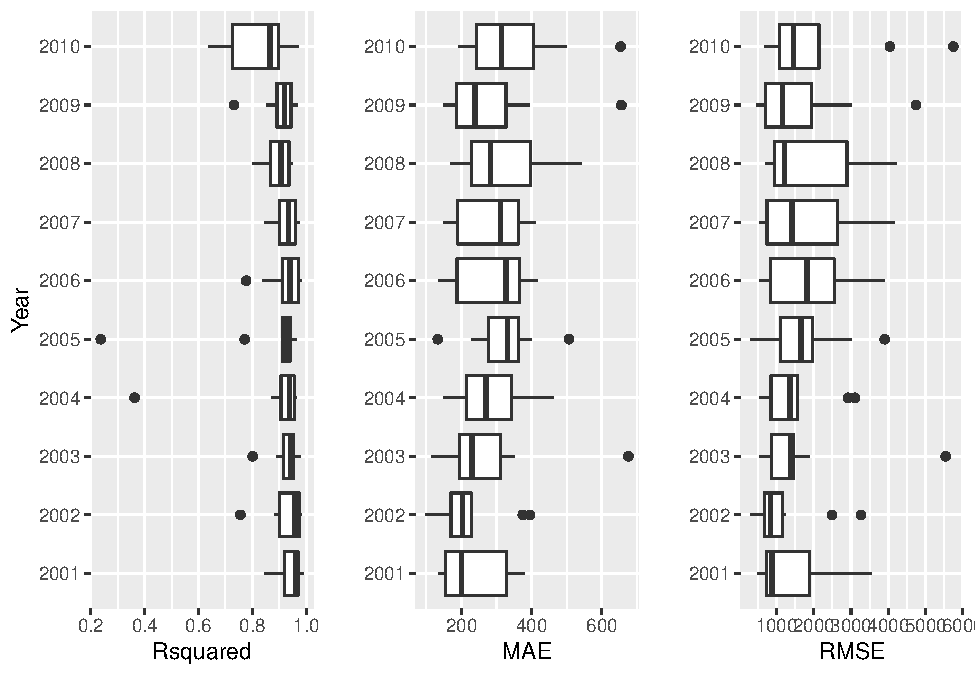
\includegraphics[width=0.6\linewidth]{hl_files/figure-latex/unnamed-chunk-1-1} \caption{\label{accuracy_insample}Accuracy metrics}\label{fig:unnamed-chunk-1}
\end{figure}

To avoid overfitting and test the predictive capacity of our models on
unseen data the models estimated using data from years \(t\) and
\(t + 1\) are aplied on years \(t + 2\). The yearly accuracy metrics are
presented in Table \ref{accuracy_test} and the predicted versus the
observed flows of interregional trade are plotted in Figure
\ref{prediction}. Indeed, our models are able to make highly accurate
out of sample predictions for interregional trade in the UK. The
R-squared only drops below \(0.9\) in 2005 and 2010 (\(0.89\) and
\(0.63\)), while it exceeds \(0.95\) in 2002 and 2004. As Figure
\ref{prediction} indicates the highest errors are observed for the
regional pairs with the two highest flows of interregional trade every
year and our models under- and overestimate their flows. These outliers
are always the intra-regional flows within Inner and Outer London
regions (UKI1 and UKI2). With the exception of these extreme values
though (trade flows above \(\pounds 50\) \(billions\)) our model perform
remarkably well in out of sample predictions. Comparing to other
attempts in the literature to predict trade flows.

\begin{table}[!htbp] \centering 
	\caption{Accuracy metrics in unseen data from t + 2\label{accuracy_test}} 
	\label{} 
	\footnotesize 
	\begin{tabular}{@{\extracolsep{0pt}} cccc} 
		\\[-1.8ex]\hline 
		\hline \\[-1.8ex] 
		year & RMSE & Rsquared & MAE \\ 
		\hline \\[-1.8ex] 
		2002 & 937.93 & 0.96 & 159.87 \\ 
		2003 & 1360.28 & 0.94 & 244.75 \\ 
		2004 & 1014.83 & 0.95 & 179.15 \\ 
		2005 & 1790.07 & 0.89 & 304.86 \\ 
		2006 & 1706.73 & 0.92 & 309.16 \\ 
		2007 & 1920.11 & 0.91 & 210.23 \\ 
		2008 & 1558.92 & 0.92 & 233.35 \\ 
		2009 & 1353.12 & 0.93 & 202.7 \\ 
		2010 & 3170.16 & 0.63 & 303.68 \\ 
		\hline \\[-1.8ex] 
	\end{tabular} 
\end{table}

\begin{figure}[p]
	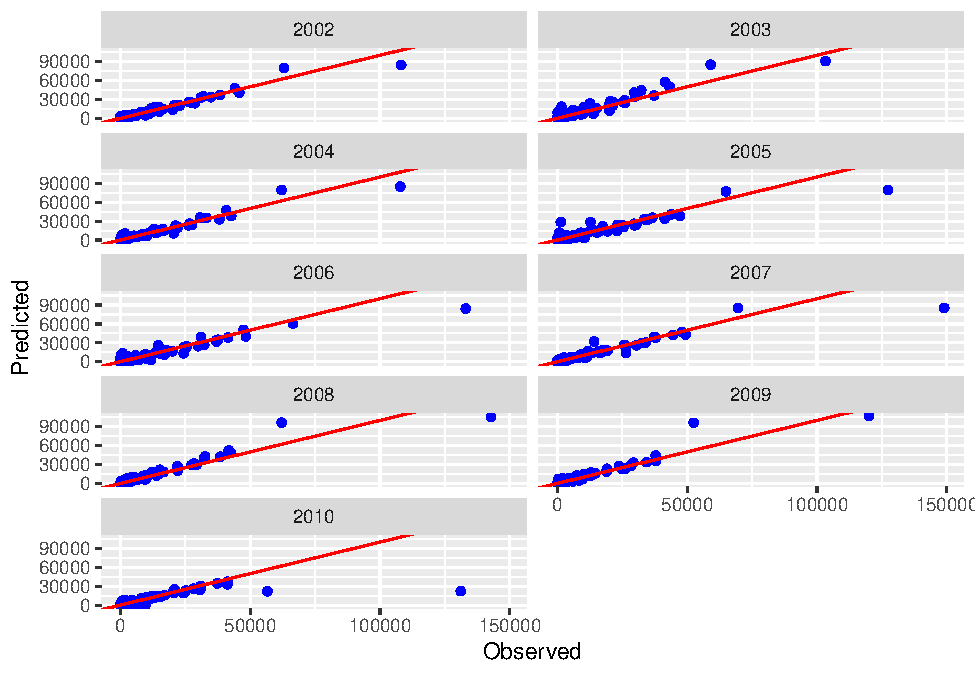
\includegraphics[width=1\linewidth]{hl_files/figure-latex/unnamed-chunk-5-1} \caption{\label{prediction}Predicted vs. observed interregional trade by year}\label{fig:unnamed-chunk-5}
\end{figure}

Our research framework enables us to disaggregate our results in terms
of economic sectors. So, we repeat the same modelling procedure for each
sector separately and Figure \ref{rsquared_sectors} reports the
R-squared values for the predictions of the unseen \(t + 2\)
interregional trade flows for each sector. As expected, our model
perform worst in specific sectors. The most obvious example is
hospitality, the R-squared for which drops below 0.25 between the
predicted and observed values for \(2004\) and \(2010\). Through the
study period though it does not exceed 0.75. A similar trend -- although
not as dramatic -- can be observed for real estate. With the exception
of \(2010\), the predictive capacity of our models is high for all the
sectors as R-squared is consistently above .075. Our models perform
exceptionally good in predicting unseen interregional trade flows
regarding manufacturing and construction as well as requirement.

\begin{figure}[p]
	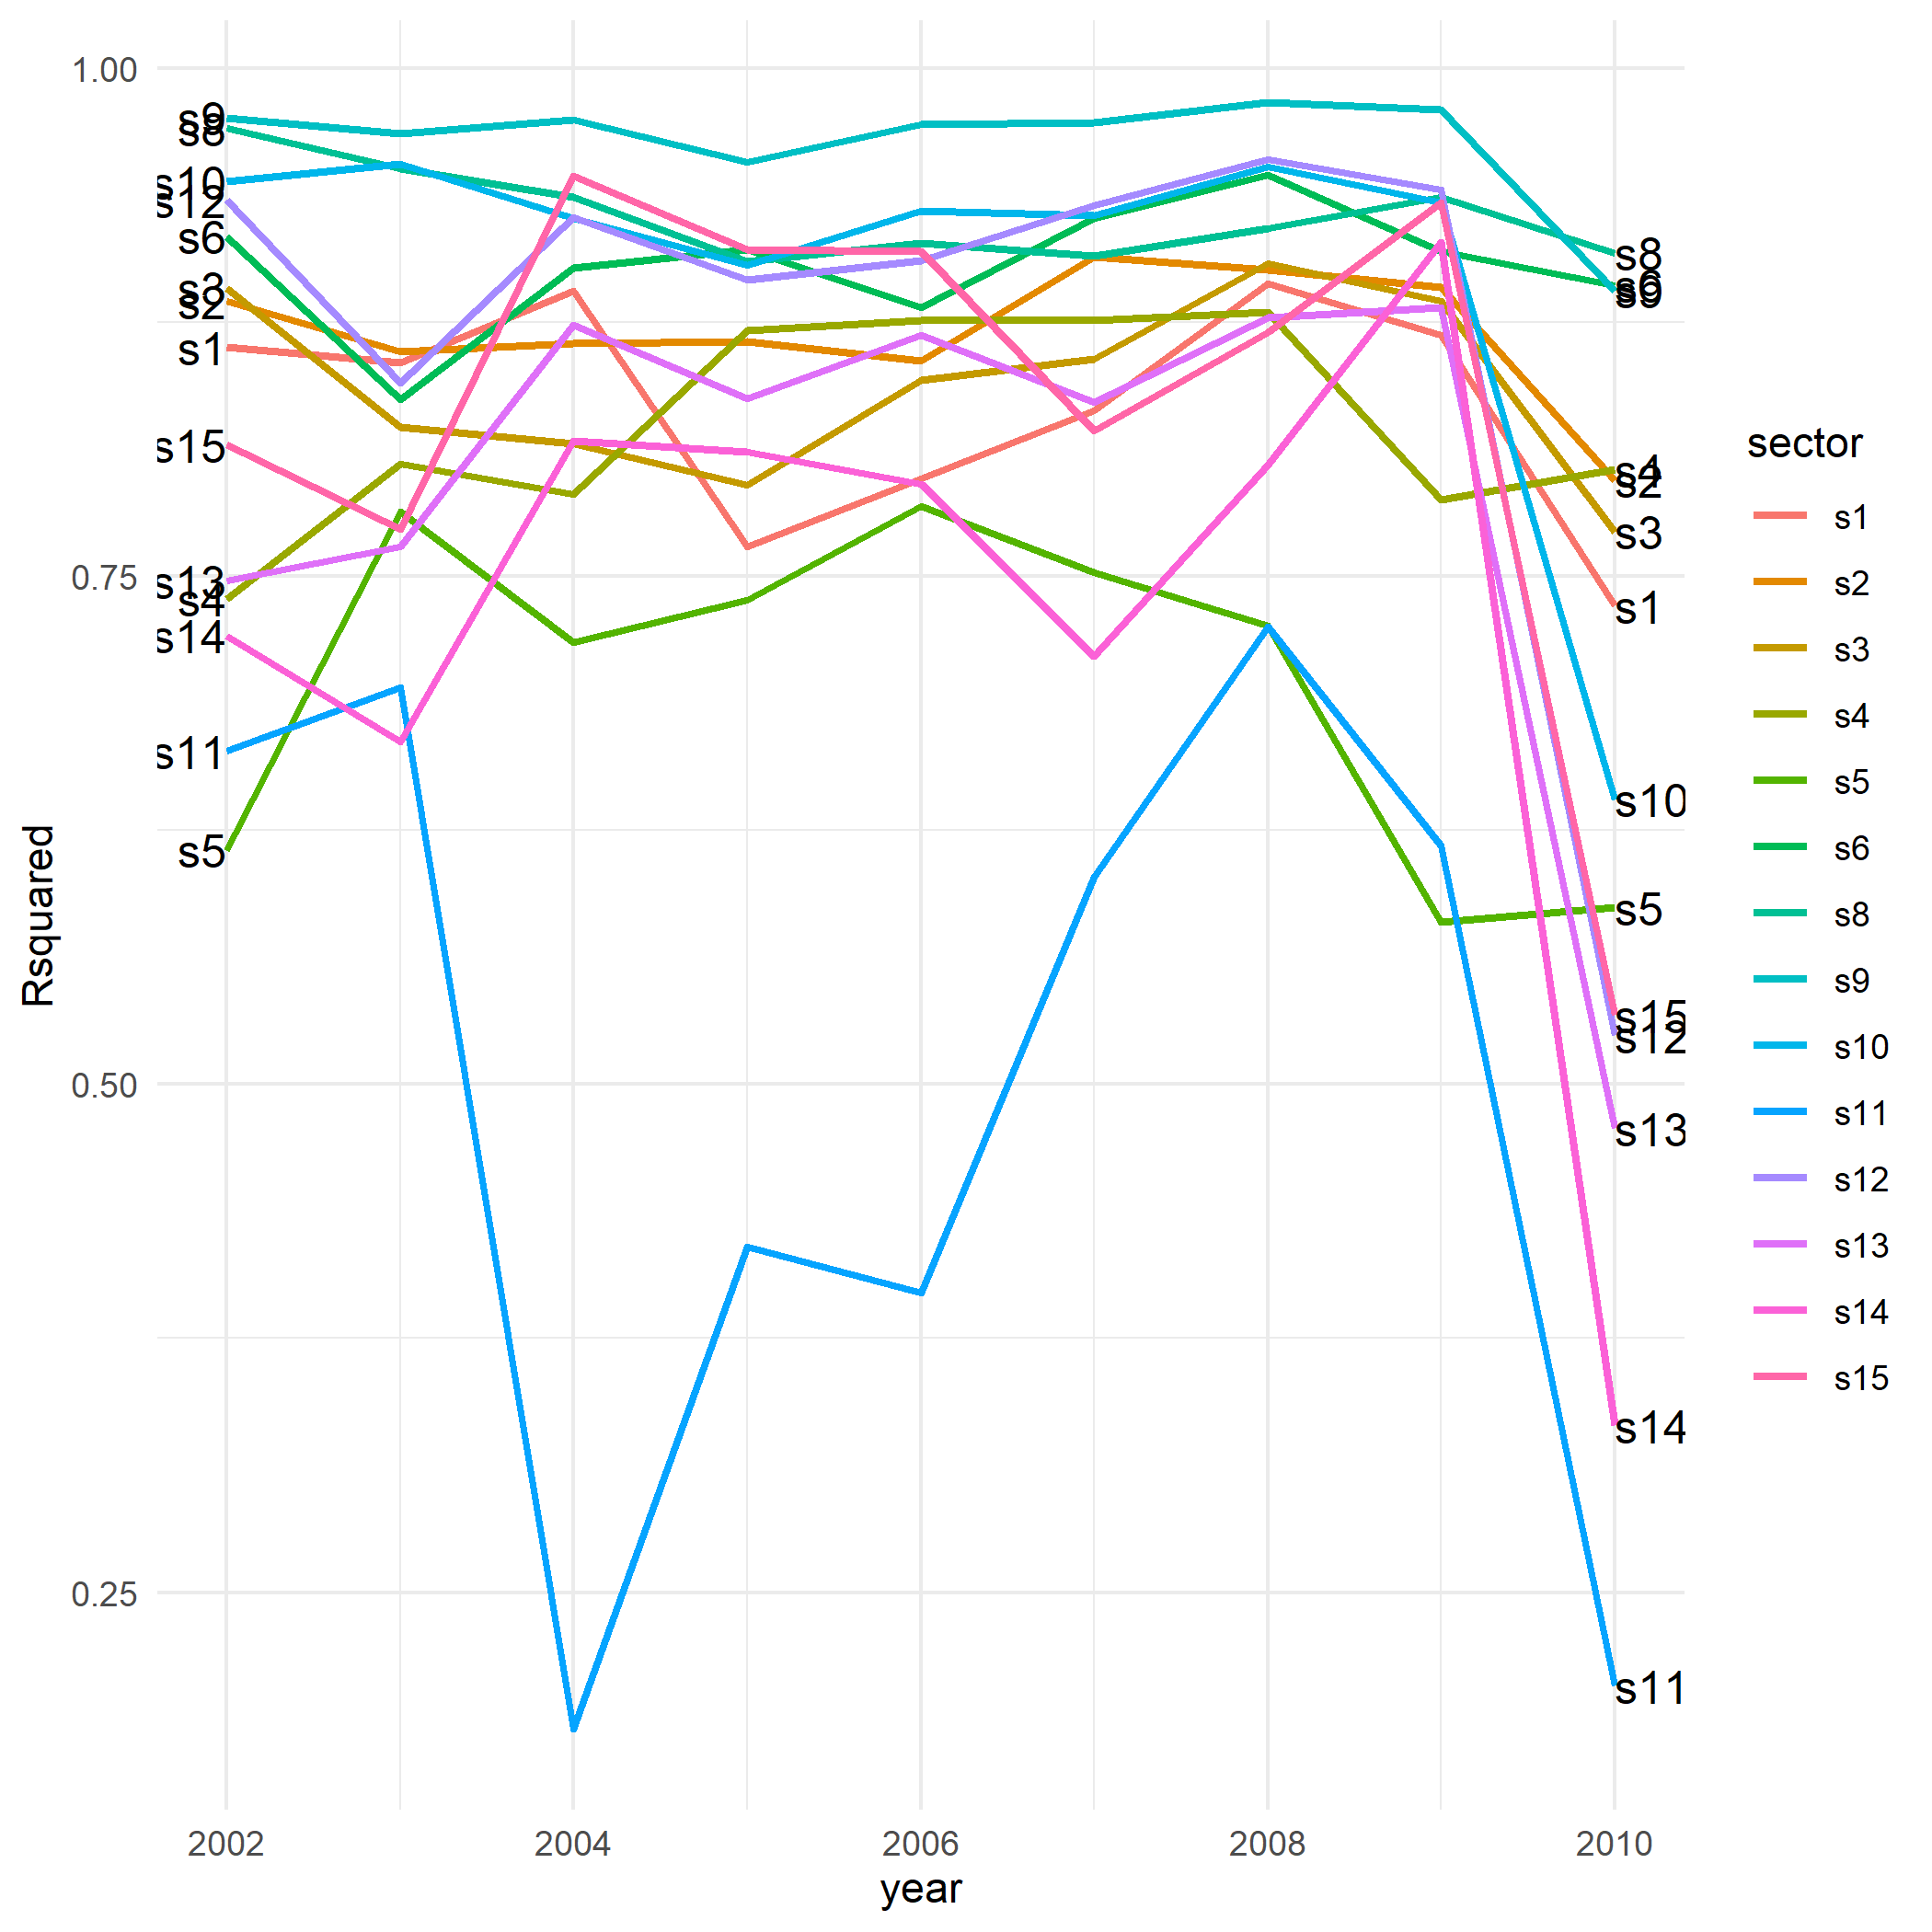
\includegraphics[width=1\linewidth]{figures/sector_rsquared} \caption{\label{rsquared_sectors}R-squared for t + 2 out of sample predictions per sector.\\\hspace{\textwidth}\tiny Notes: s1: Agriculture, s2: Mining, s3: Food, s4: Textiles, s5: Chemicals, s6: Equipment, s8: Manufacturing; s9: Construction, s10: Distribution, s11: Hospitality, s12:  Transport, s13: Financial, s14: Real Estate, s15: Non-Market Services.}\label{fig:unnamed-chunk-7}
\end{figure}

To further assess the role of our main variable of interest -- the
volume of hyperlinks between regions -- in predicting interregional
trade flows we estimate the first set of models for the total trade
flows using alternative specifications. Firstly, we exclude the distance
or the hyperlinks features. The accuracy metrics for the out of sample
predictions for unseen trade flow data from years \(t + 2\) are
presented in Figure \ref{alt.accuracy}, which also includes the metrics
for the base models presented in Table \ref{accuracy_test} for direct
comparison. The main message from Figure \ref{alt.accuracy} is that
distance plays the most important role in predicting interregional trade
flows. All three metrics are worst when the distance is excluded. This
is not surprising as the role of distance in predicting trade and other
types of spatial interactions has been extensively highlighted in the
literature discussed in Sections \protect\hyperlink{sec:1}{1} and
\protect\hyperlink{sec:2}{2}. What is interesting though is that the gap
in terms of the prediction accuracy between the models with and without
distance decreases over time. This illustrates that over time, as the
adoption rate of web technologies increased, interregional trade flows
started leaving more `digital breadcrumbs' behind and, therefore, are
better reflected in the volumes of interregional hyperlinks
\citep{rabari_storper2014}. Nevertheless, the predictive capacity of
distance remains unchallenged at large as the green lines in Figure
\ref{alt.accuracy} indicate.

\begin{figure}[p]
	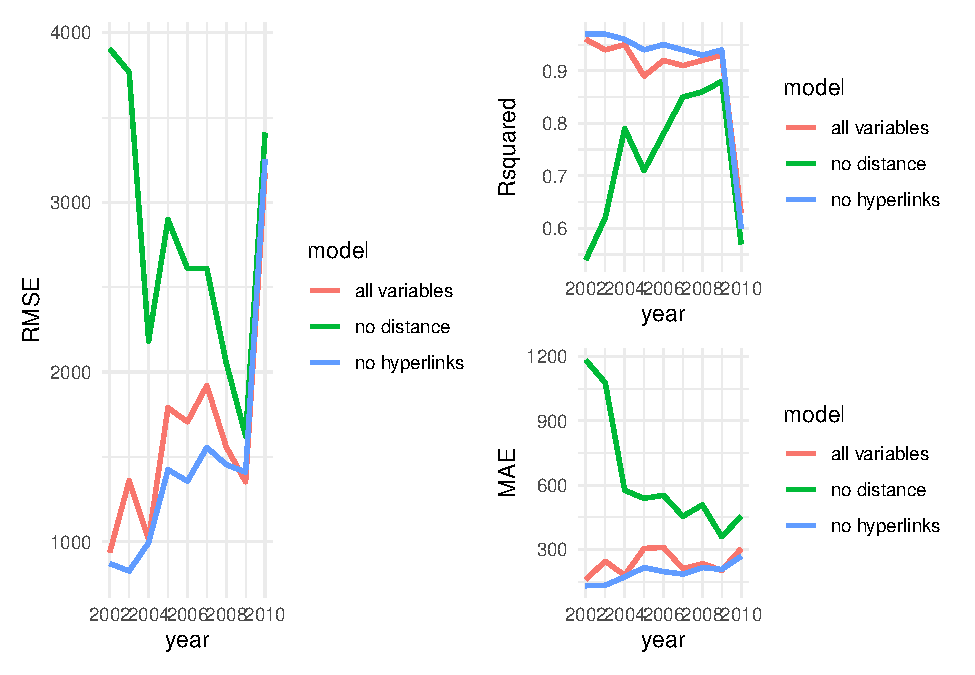
\includegraphics[width=1\linewidth]{hl_files/figure-latex/unnamed-chunk-9-1} \caption{\label{alt.accuracy}Accuracy metrics for alternative specifications}\label{fig:unnamed-chunk-9}
\end{figure}

To further assess the robustness of our results, we repeat our workflow
for a different sample of websites. Instead of including only the
websites with a unique postcode, we add in our sample websites with up
to \(11\) unique postcodes. As discussed in Section
\protect\hyperlink{sec:4}{4}, this enhanced sample of websites
containing multiple postcodes within the web text represents commercial
websites with multiple locations. Given that we are not able to
distinguish the role of these different locations we expect that using
this sample for training and testing our models will lead to more noise.
Nevertheless, the predictive capacity of our models remains almost
unchanged according to the out of sample prediction metrics, which are
reported in Table \ref{accuracy_test_multi_pc} and the predicted versus
the observed interregional trade flows, which are plotted in Figure
\ref{prediction_multi_pc}. Indeed, R-squared drops below \(0.90\) for
only two years (\(2009\) and \(2010\)). Again, the largest prediction
errors can be easily linked to the regional pairs with the highest
volume of regional trade -- that is the London intra-regional trade.

\begin{table}[!htbp] \centering 
	\caption{Accuracy metrics in unseen data with multiple postcodes from t + 2\label{accuracy_test_multi_pc}} 
	\label{} 
	\footnotesize 
	\begin{tabular}{@{\extracolsep{0pt}} cccc} 
		\\[-1.8ex]\hline 
		\hline \\[-1.8ex] 
		year & RMSE & Rsquared & MAE \\ 
		\hline \\[-1.8ex] 
		2002 & 1181.91 & 0.94 & 244.27 \\ 
		2003 & 1428.99 & 0.93 & 282.77 \\ 
		2004 & 1011.14 & 0.95 & 173.31 \\ 
		2005 & 1414.77 & 0.94 & 232.25 \\ 
		2006 & 1433.92 & 0.94 & 208.32 \\ 
		2007 & 1894.59 & 0.91 & 227.77 \\ 
		2008 & 1206.3 & 0.95 & 249.66 \\ 
		2009 & 2008.83 & 0.81 & 238.38 \\ 
		2010 & 2500.1 & 0.78 & 298.27 \\ 
		\hline \\[-1.8ex] 
	\end{tabular} 
\end{table}

\begin{figure}[p]
	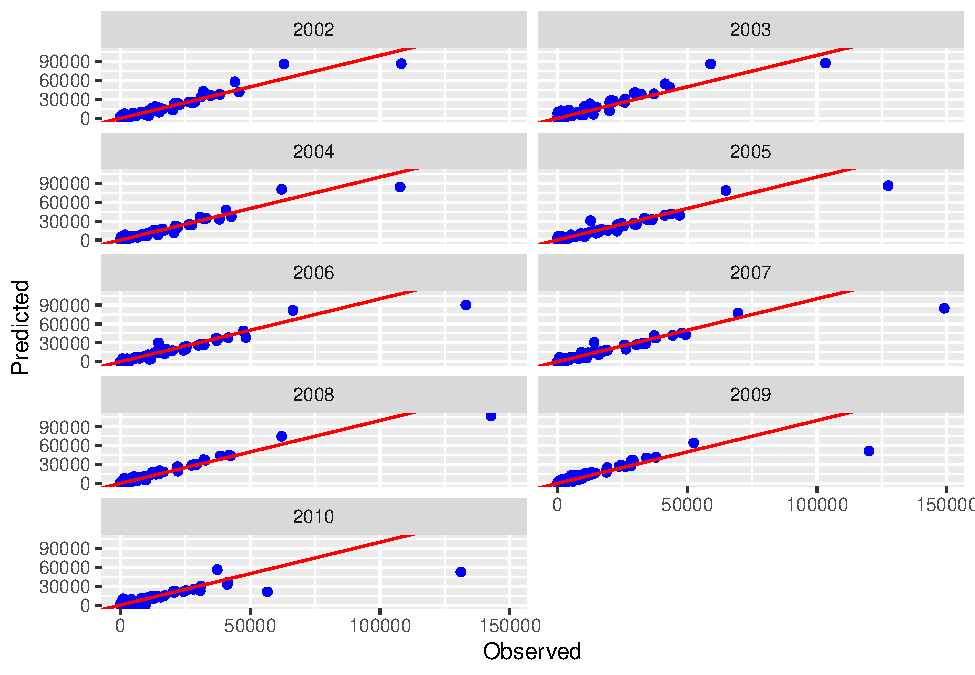
\includegraphics[width=1\linewidth]{hl_files/figure-latex/unnamed-chunk-11-1} \caption{\label{prediction_multi_pc}Predicted vs. observed interregional trade by year for multiple postcodes}\label{fig:unnamed-chunk-11}
\end{figure}

\hypertarget{sec:6}{%
	\section{Conclusions}\label{sec:6}}

In summary, it is very well established in the literature that
interregional trade is difficult to capture. The current state of the
art of empirical studies focusing on modelling international trade tend
to be explanatory in their nature and most attempts to produce
disaggregated interregional trade flows are mostly based on pure
distance decay measures. This paper proposes the use of innovative and
openly accessible web data within a state-of-the art ML framework to
predict such trade flows. The predictive capacity of our model is very
good and it is indicative of the \emph{digital} paper trail that trade
leaves behind. Our framework could be utilised in framework to produce
such interregional data, which otherwise would be very difficult to
capture, and also produce these data at much more disaggregated scales
than before.

\section{References}

\bibliographystyle{ACM-Reference-Format}
\bibliography{bibliography}

\end{document}